\documentclass[border=10pt]{standalone}
\usepackage[svgnames]{xcolor}
\usepackage{amsmath}
\usepackage{pgfplots}
\pgfplotsset{compat=newest}
\usepackage[sfdefault]{FiraSans}
\usepackage{FiraMono}
\renewcommand*\familydefault{\sfdefault}
\begin{document}
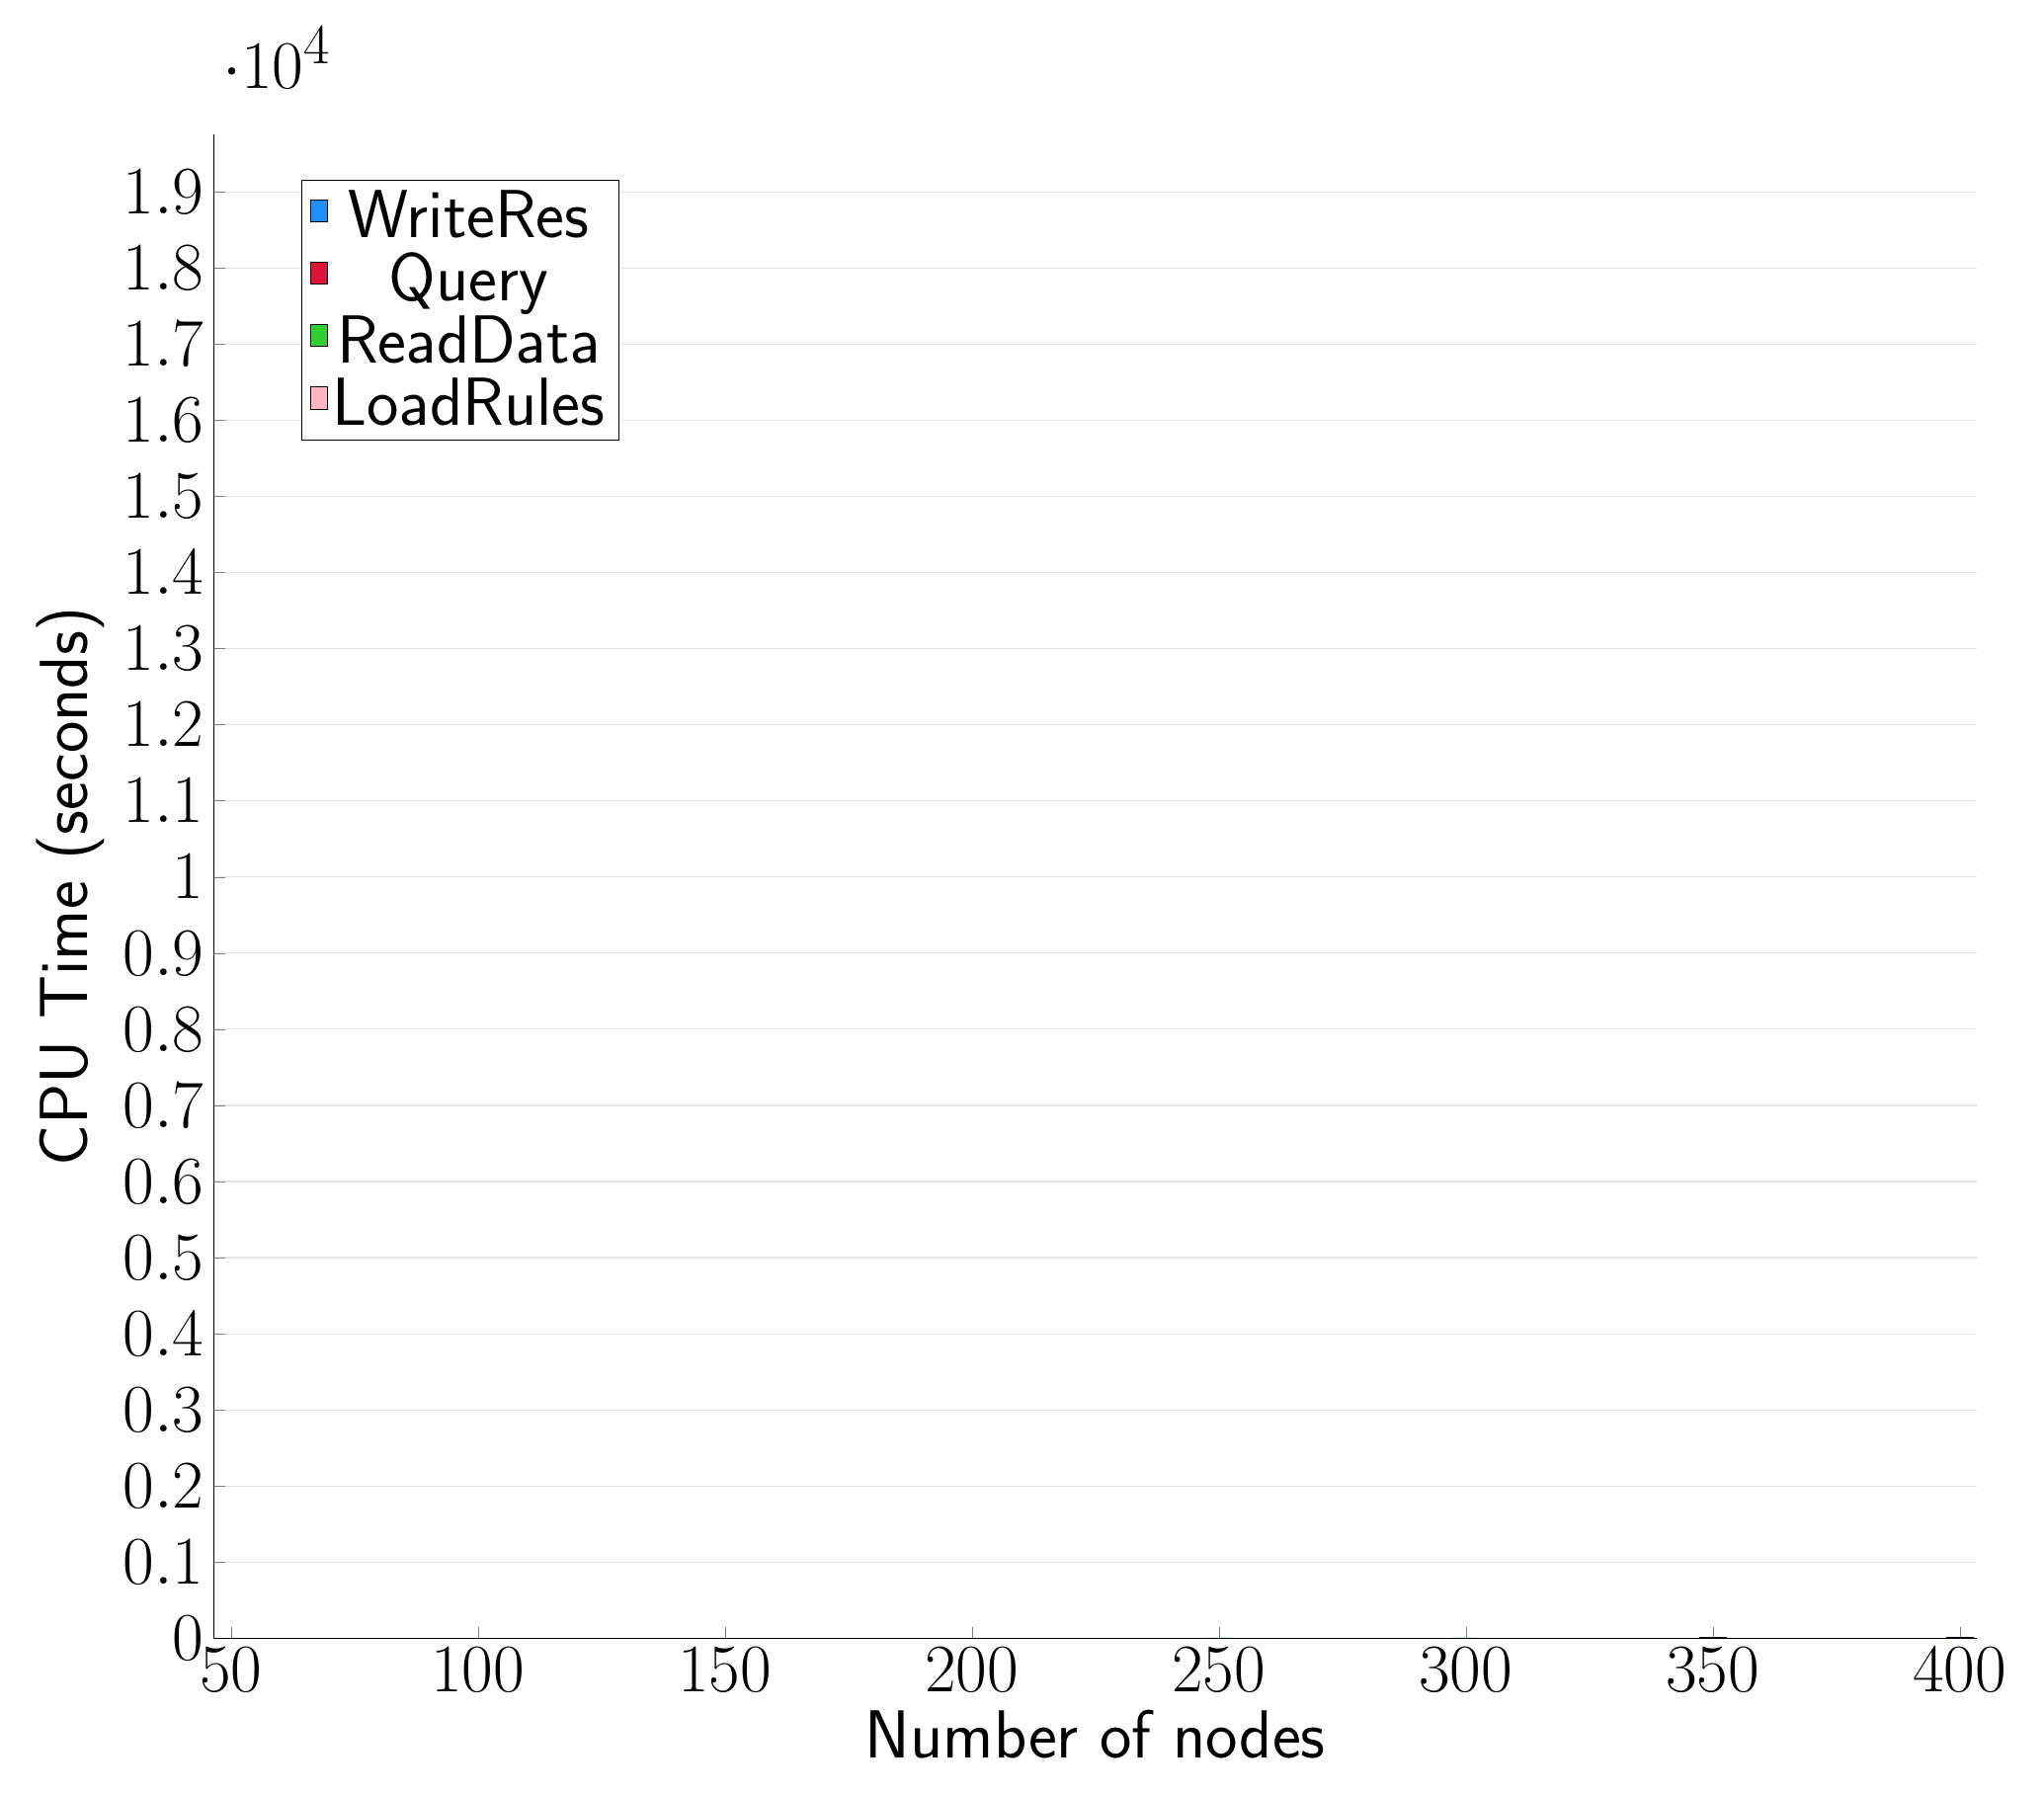
\begin{tikzpicture}
\begin{axis}[
   ybar stacked,
   width=2\textwidth,
   bar width=0.35cm,
   ymajorgrids, tick align=inside,
   major grid style={draw=gray!20},
   xtick=data,
   ymin=0, ymax=19758.773333333433,
   axis x line*=bottom,
   axis y line*=left,
   enlarge x limits=0.01,
   legend style={
       at={(0.23, 0.97)},
       anchor=north east,
       legend columns=1,
       font=\Huge,
   },
   ylabel={CPU Time (seconds)},
   xlabel={Number of nodes},
   label style={font=\Huge},
   tick label style={font=\Huge},
]
\addlegendimage{fill=DodgerBlue, draw=black, line width=0.2pt}
\addlegendentry{WriteRes}
\addlegendimage{fill=Crimson, draw=black, line width=0.2pt}
\addlegendentry{Query}
\addlegendimage{fill=LimeGreen, draw=black, line width=0.2pt}
\addlegendentry{ReadData}
\addlegendimage{fill=LightPink, draw=black, line width=0.2pt}
\addlegendentry{LoadRules}
\addplot +[fill=LightPink, draw=black, line width=0.2pt] coordinates {
(50, 0.003408666666666667)
(100, 0.00420033333333333)
(150, 0.0030189999999999995)
(200, 0.0028553333333333334)
(250, 0.0031286666666666667)
(300, 0.0033333333333333335)
(350, 0.0031806666666666667)
(400, 0.00336566666666667)
};
\addplot +[fill=LimeGreen, draw=black, line width=0.2pt] coordinates {
(50, 0.027361999999999997)
(100, 0.09817133333333333)
(150, 0.20490966666666666)
(200, 0.41593233333333335)
(250, 0.5655023333333333)
(300, 0.8820236666666667)
(350, 1.2247656666666666)
(400, 1.9457556666666669)
};
\addplot +[fill=Crimson, draw=black, line width=0.2pt] coordinates {
(50, 0.015841333333333332)
(100, 0.11494733333333333)
(150, 0.3373923333333333)
(200, 0.8351596666666666)
(250, 1.6271713333333333)
(300, 2.8277180000000004)
(350, 4.644032333333333)
(400, 13.368732333333334)
};
\addplot +[fill=DodgerBlue, draw=black, line width=0.2pt] coordinates {
(50, 0.07406533333333333)
(100, 0.32948133333333335)
(150, 0.728805)
(200, 1.046429)
(250, 1.8803869999999998)
(300, 2.5208250000000003)
(350, 3.723563)
(400, 2.193531)
};
\end{axis}
\end{tikzpicture}

\end{document}
